{
\begin{figure}[th]
\centering
\begin{center}
\centerline{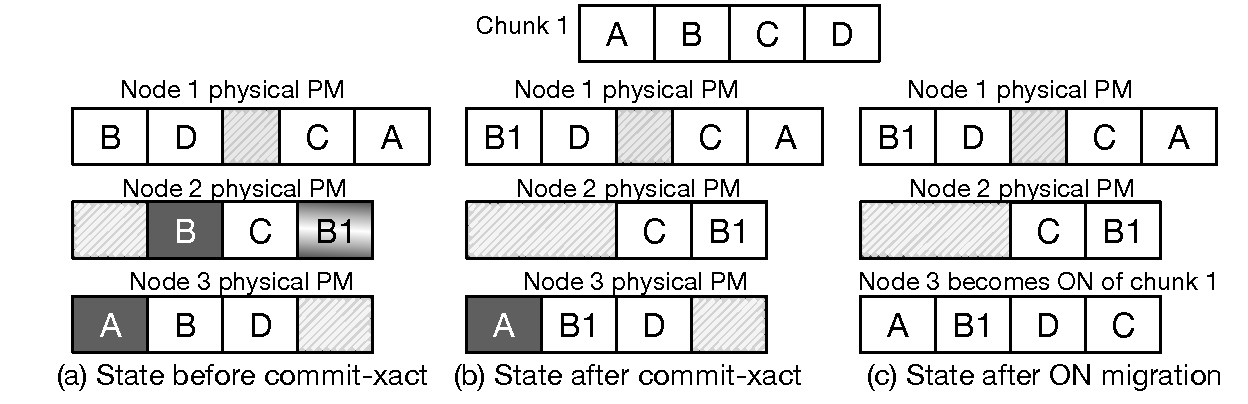
\includegraphics[width=\columnwidth]{Figures/data-eg.pdf}}
\end{center}
\vspace{-0.2in}
\mycaption{fig-data-eg}{Data State Change Example.}
{
White, black, and striped blocks represent \committed, \redundant, and \dirty\ states.
Before commit, Node 2 and Node 3 both have cached copies of 
data page $B$. Node 2 has written to $B$ and created a \dirty\ page, $B1$.
During commit, Node 2 pushes the content $B1$ to its \on, Node 1.
Node 1 updates its \committed\ copy to $B1$ and also sends this update to Node 3.
Figure (c) shows the state after migrating the \on\ of chunk 1 from Node 1 to Node 3. 
%page $A$ on Node 3 is \redundant.
After migration, Node 3 has all the pages of the chunk and all of them are in \committed\ states.
}
\vspace{-0.1in}
\end{figure}
}
